\apendice{Documentación técnica de Usuario }

\section{Requisitos previos}
\subsection{Modo usuario}
De forma previa a la utilización de la aplicación, se deberá tener instalado en el equipo lo siguiente: 
\begin{itemize}
\item \textbf{Sistema operativo}
\begin{itemize}
\item Windows
\end{itemize} 
\item \textbf{distribución}
\begin{itemize}
\item Anaconda en su última versión estable 5.6, con la versión de Python 3.6. Dicha descarga se puede realizar a través del siguiente enlace: \url{https://www.anaconda.com/download/}
\end{itemize}
\item \textbf{Librerías auxiliares}
\begin{itemize}
\item Matplotlib en la versión 2.0 o superior. En caso de no disponer de dicha librería actualizada, se puede actualizar con el siguiente comando: "conda update --all".
\end{itemize}
\item \textbf{Proyecto}
\begin{itemize}
\item Descargar o clonar el proyecto TFG-Sistema\_de\_recomendacion\_Asignaturas\_Optativas a través del siguiente enlace: \url{https://github.com/ClaraPalacios/TFG-Sistema_de_recomendacion_Asignaturas_Optativas/issues}
\end{itemize}
\end{itemize}

\subsection{Modo administrador}
En el modo administrador, además, será necesario el acceso a la API de GoogleDrive, de forma que serán necesario: 
\begin{itemize}
\item \textbf{Sistema operativo}
\begin{itemize}
\item Windows
\end{itemize} 
\item \textbf{distribución}
\begin{itemize}
\item Anaconda en su última versión estable 5.6, con la versión de Python 3.6. Dicha descarga se puede realizar a través del siguiente enlace: \url{https://www.anaconda.com/download/}
\end{itemize}
\item \textbf{Librerías auxiliares}
\begin{itemize}
\item Matplotlib en la versión 2.0 o superior.  En caso de no disponer de dicha librería actualizada, se puede actualizar con el siguiente comando: "conda update --all".
\end{itemize}
\item \textbf{Datos Auxiliares}
\begin{itemize}
\item Clave secreta importada en el fichero JSON. 
\end{itemize}
\item \textbf{Proyecto}
\begin{itemize}
\item Descargar o clonar el proyecto TFG-Sistema\_de\_recomendacion\_Asignaturas\_Optativas a través del siguiente enlace: \url{https://github.com/ClaraPalacios/TFG-Sistema_de_recomendacion_Asignaturas_Optativas/issues}
\end{itemize}
\end{itemize}

\section{Ejecución del proyecto}


\section{Utilización}
Tras la ejecución del proyecto, se abrirá una pestaña en la que el usuario debe introducir su correo y contraseña. 
\subsection{Primera ventana}

\subsection{Segunda ventana}
Tras iniciar sesión, aparecerá la siguiente pestaña: \ref{fig:E.2.1}
\begin{figure}[h]
\centering
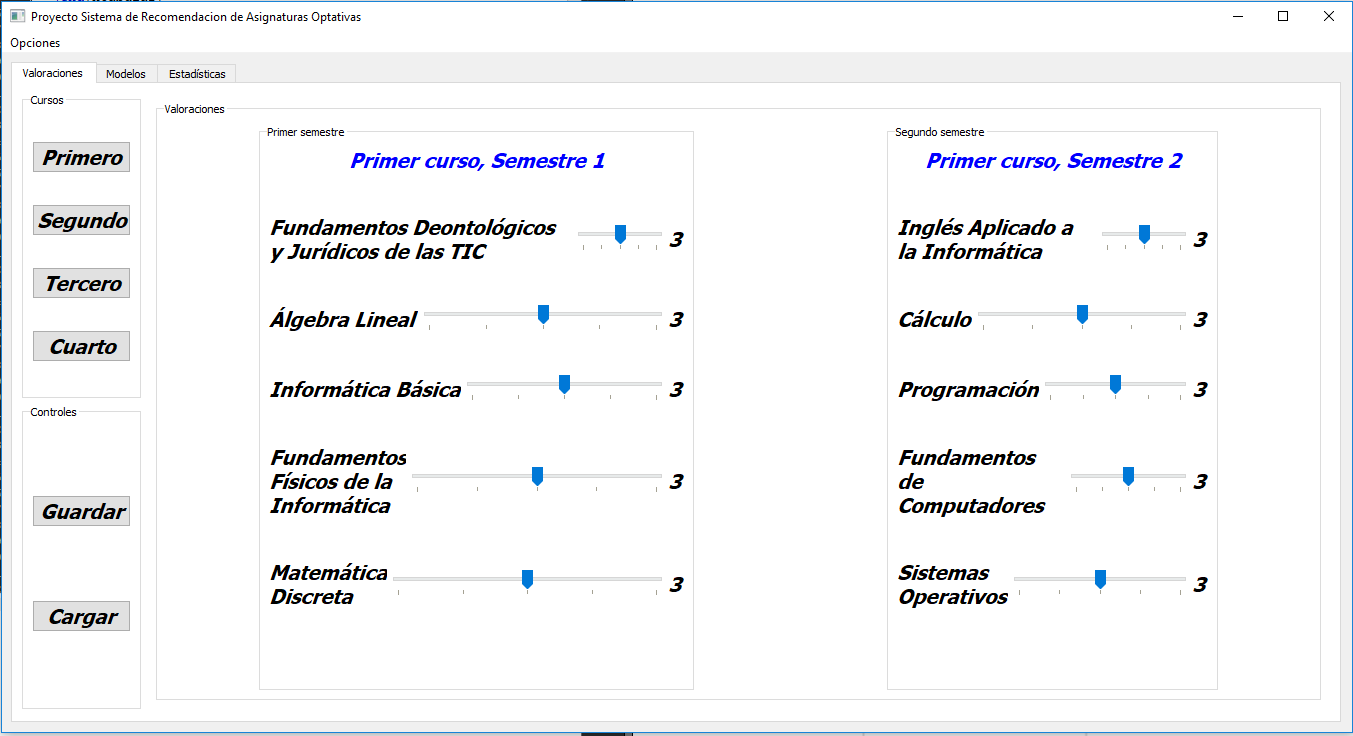
\includegraphics[width=0.90\textwidth]{INTERFAZ_Rellenado_Datos_V1-0}
\caption{Interfaz de rellenado de cuestionario}
\label{fig:E.2.1}
\end{figure}
Los cursos, son botones clicables, los cuales, al ser pulsados, muestran las asignaturas correspondientes a dicho año. \ref{fig:E.2.2}
\begin{figure}[h]
\centering
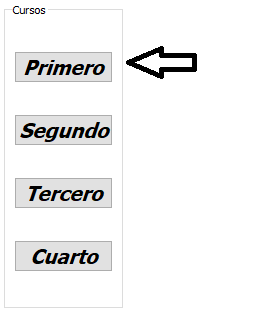
\includegraphics[width=0.90\textwidth]{cursos}
\caption{Cursos}
\label{fig:E.2.2}
\end{figure}

En caso de haberse registrado por primera vez, en el área central de la pantalla, las asignaturas constarán de valores medios, que deberán ser modificados por el usuario. \ref{fig:E.2.3}
\begin{figure}[h]
\centering
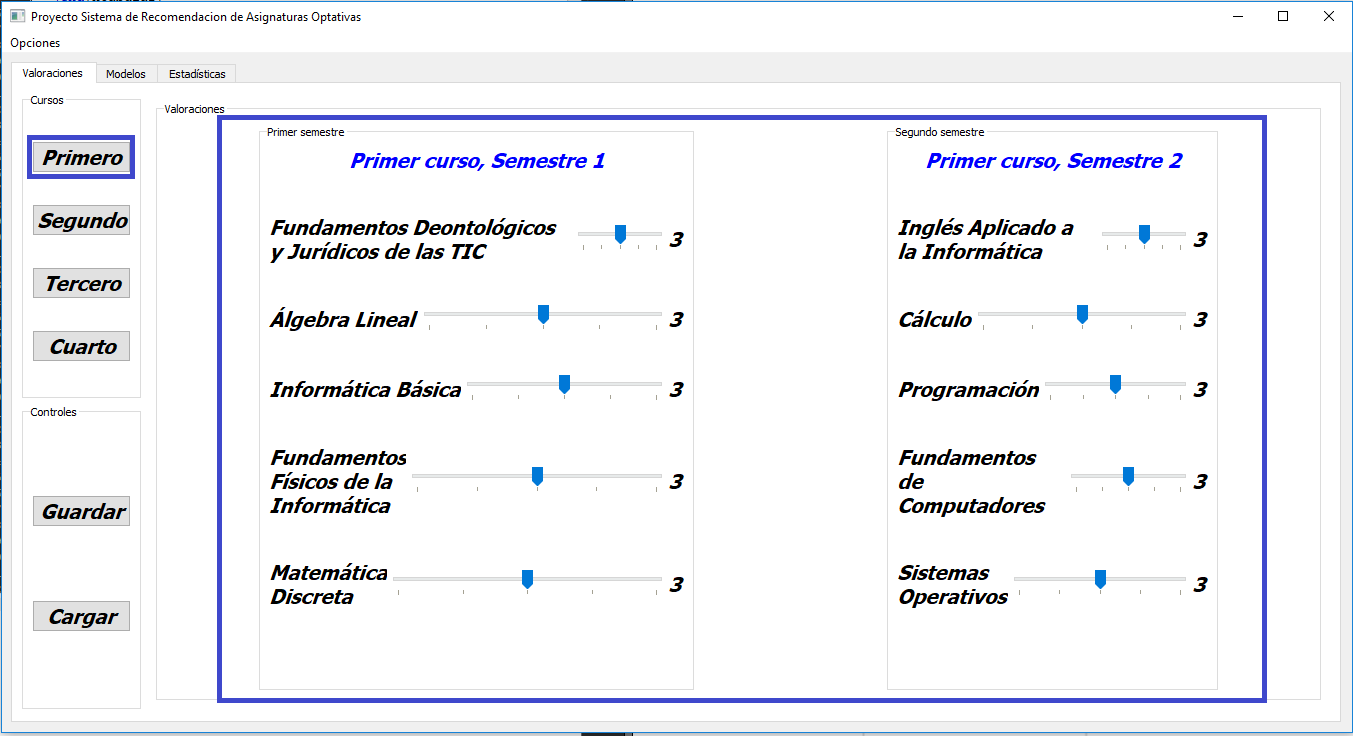
\includegraphics[width=0.90\textwidth]{INTERFAZ_Rellenado_Datos_Central_V1-0}
\caption{Parte central pestaña rellenado de datos}
\label{fig:E.2.3}
\end{figure}
Se pueden modificar tanto con el ratón, arrastrando  slider o bien con el teclado con las flechas izquierda y derecha. En la siguiente imagen se puede observar la diferencia entre utilizar el ratón y el teclado. \ref{fig:E.2.4}
\begin{figure}[h]
\centering
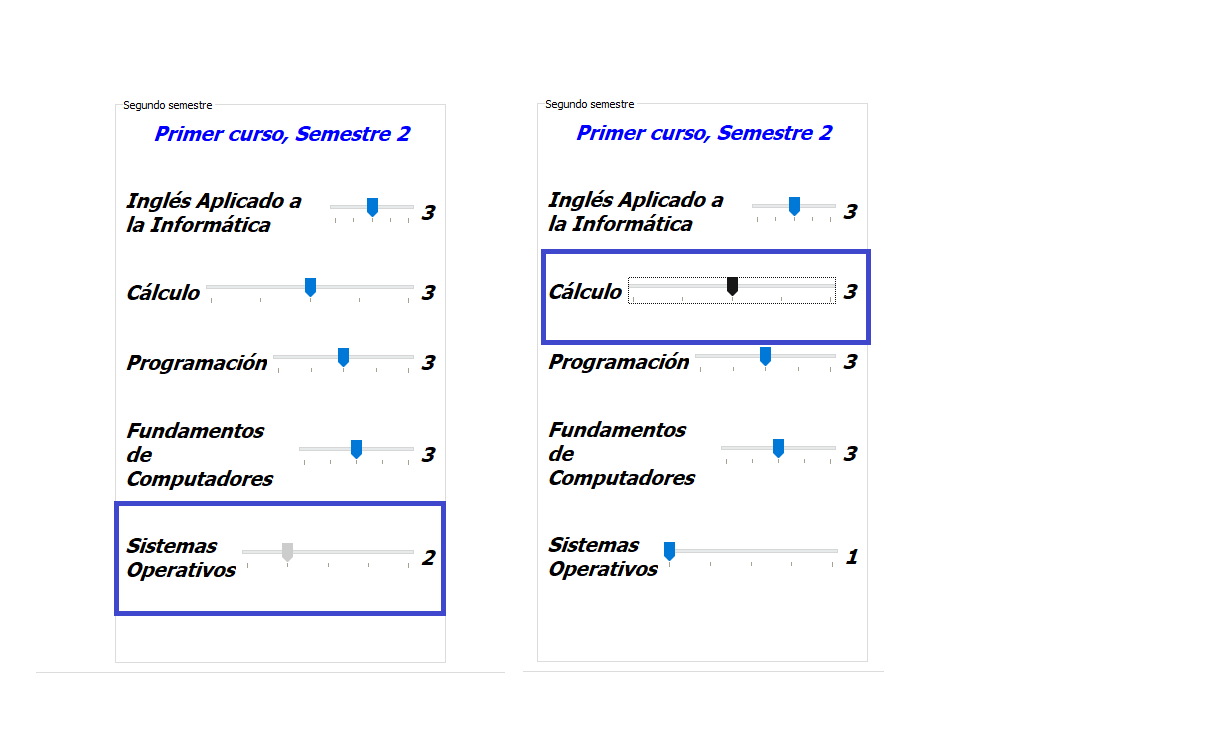
\includegraphics[width=0.90\textwidth]{INTERFAZ_Rellenado_Datos_Raton_V1-0}
\caption{Img Izq: Selección con ratón. Img Der: Selección con teclado}
\label{fig:E.2.4}
\end{figure}
